\documentclass[a4paper,10pt]{jsarticle}
%\documentclass[a4paper,10pt]{jsbook}

\usepackage[dvipdfmx]{graphicx, color}
%\usepackage{folha}
\graphicspath{{image/}}

\usepackage{color}
\usepackage{array}
\usepackage{longtable}
\usepackage{alltt}
\usepackage{graphics}
\usepackage{vpp-nms}
%\usepackage{vpp}
\usepackage{makeidx}
\makeindex

\usepackage{colortbl}

\usepackage[dvipdfmx,bookmarks=true,bookmarksnumbered=true,colorlinks,plainpages=true]{hyperref}

%\AtBeginDvi{\special{pdf:tounicode 90ms-RKSJ-UCS2}}
\AtBeginDvi{\special{pdf:tounicode EUC-UCS2}}

\definecolor{covered}{rgb}{0,0,0}      %black
\definecolor{not-covered}{rgb}{1,0,0}  %red

\setcounter{secnumdepth}{6}
\makeatletter
\renewcommand{\paragraph}{\@startsection{paragraph}{4}{\z@}%
  {1.5\Cvs \@plus.5\Cdp \@minus.2\Cdp}%
  {.5\Cvs \@plus.3\Cdp}%
  {\reset@font\normalsize\bfseries}}
\makeatother

\renewcommand{\sf}{\sffamily \color{blue}}

\newcommand{\syou}{\texttt{<}}
\newcommand{\dai}{\texttt{>}}

%\include{Title}

%\pagestyle{empty}
\usepackage{fancyhdr}
\usepackage{lastpage} 
  \pagestyle{fancy} 
   \let\origtitle\title 
  \renewcommand{\title}[1]{\lfoot{#1}\origtitle{#1}}

  \rfoot{\today}
  \rhead{[\ \scshape\oldstylenums{\thepage}\ / %
      \scshape\oldstylenums{\pageref{LastPage}}\ ]}
  \cfoot{}


\begin{document}

% the title page
\title{エクスプレス予約システムの問題点を推測し、修正した仕様}
\author{佐原 伸\\\\
法政大学\\
情報科学研究所\\
}
%\institute{\pgldk \and \chessnl}
\date{\mbox{}}
\maketitle

%\TaoReport{ガードコマンド・モデル}{\today}{タオベアーズ}{佐原伸}
%\setlength{\baselineskip}{12pt plus .1pt}
%\tolerance 10000
\tableofcontents
%\thispagestyle{empty} 

%\include{Abstract}
\section {はじめに}
鉄道会社Aの特急券予約システムに関する
「特急券予約システムシステムの問題点を推測した仕様」(第\ref{VDMModelExpressReservation}章参照)を、
本来あるべき仕様として書き直した仕様である。

\subsection{本来どうすべきだったのか?}
修正後のクラス図\ref{fig:EvolvedExpressReservationModifiedClassDiagram}で見るように、
本来、特急券予約システムは契約\footnote{口座と言ってもよいが、本モデルでは契約という名前にした}
とリンクが設定されているべきであり、
契約がクレジットカードとリンクしているべきである。

予約会員証も契約を介してクレジットカードを参照できるようにすべきである。

\begin{figure}[h]
	\centering
	{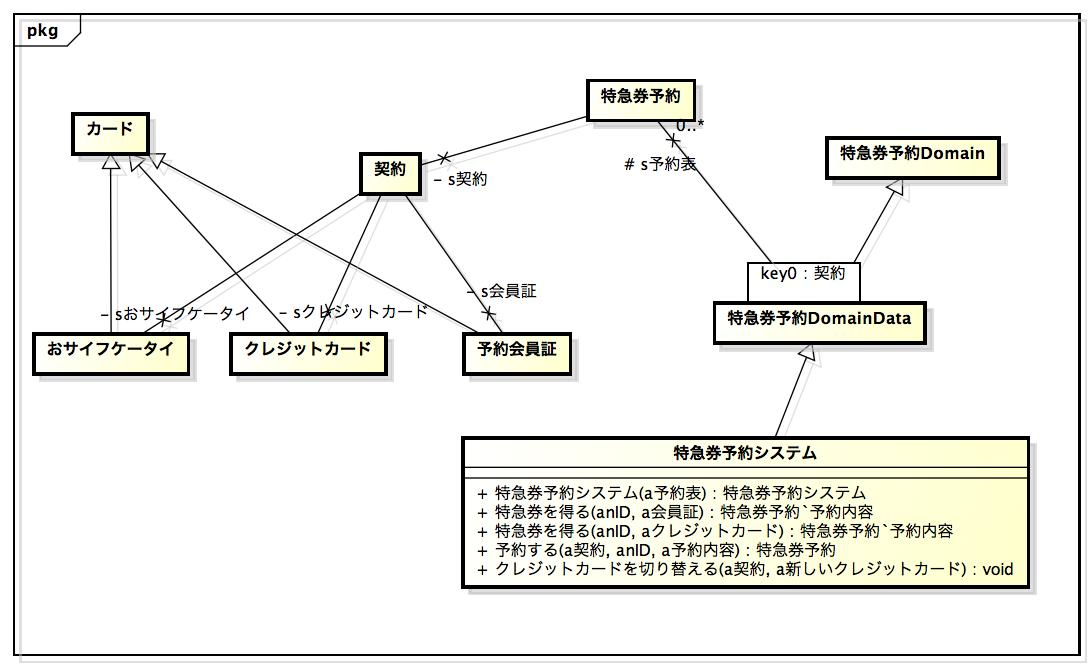
\includegraphics[width=55zw, keepaspectratio]{./EvolvedExpressReservation/image/ModifiedClassDiagram.jpg}}
	\caption{修正後のクラス図}
	\label{fig:EvolvedExpressReservationModifiedClassDiagram}
	\index{しゆせいこのくらすす@修正後のクラス図}
\end{figure}

このようにしておけば、契約に変更があっても、古い特急券予約は新しい契約を介して、新しいクレジットカードにアクセスでき、
同じく予約会員証も新しいクレジットカードにアクセスできる。

修正前のクラス図\ref{fig:ExpressReservationClassDiagram}
と比べれば、再利用性と保守性が増しているにもかかわらず、
構造自体は特に複雑になっているわけではないことが分かる。
	
\include{ReservationSysytem.vpp}	
\include{Common.vpp}
\include{ReservationDomain.vpp}
\include{ReservationDomainData.vpp}
\include{ExpressReservatiopn.vpp}
\include{Contract.vpp}
\include{Card.vpp}
\include{CredirCard.vpp}
\include{CustomerCard.vpp}
\include{SUICA.vpp}
\include{MyTest.vpp}
\include{MyTestCase.vpp}
\section{まとめ}
\subsection{統計情報}
注釈抜きのVDM++ソース行数は、492行、
モデル作成工数は約1日、発表用の資料作成とVDM++モデルの読みやすさのための整形・清書に約2日かかった。

なお、上記モデルの作成工数は、筆者が問題を解決するために消費した工数より少ない。

%\begin{thebibliography}{9}
\section{参考文献等}
VDM++\cite{Kyushu2016PPE}は、
1970年代中頃にIBMウィーン研究所で開発されたVDM-SL\cite{Kyushu2016SLE}を拡張し、
さらにオブジェクト指向拡張したオープンソースの形式仕様記述言語である。
\bibliographystyle{jplain}
%\bibliography{/Users/sahara/svnw/sahara}
\bibliography{/Users/sahara/Dropbox/bib/saharaUTF8}
%\bibliography{/Users/ssahara/svnwork/sahara}

%\end{thebibliography}

%\newpage
%\addcontentsline{toc}{section}{Index}
\printindex

\end{document}
